% Chapter Template

\chapter{User studies} % Main chapter title

\label{Chapter6} % Change X to a consecutive number; for referencing this chapter elsewhere, use \ref{ChapterX}

\lhead{Chapter 6. \emph{User experience evaluation}} 
Human-Robot Interaction being a rapidly advancing area of research, there is a growing need for strong experimental designs and methods of evaluation. This will bring credibility and validity to scientific research that involves humans as subjects, as recognized in the psychology and social science fields. As robots are becoming more prevalent, accurate methods to assess how humans respond to robots, how they feel about their interactions with robots, and how they interpret the actions of robots are very important. Indriya platform being aimed at naive users it is very important to evaluate how people feel about the system. In this chapter, the experiment design process, data collection and analysis are discussed.

\section{Experiment protocol}
The interaction design process suggested in \cite{Rogers2011} has been followed. The main aspects of the experiment are as follows
\begin{itemize}
\item Identifying the participants: A set of participants were identified who have beginner to intermediate level programming skill to evaluate the platform
\item Relationship with participants: A professional relationship is maintained with the participants in order to reduce the bias in the evaluation process
\item Setting goals: The main goals of the experiment considered are
\begin{itemize}
\item Whether the participants understand the objective of the system?
\item Whether the participants able to use the system?
\item Whether the participants able to execute the designed scenario on the real robot?
\end{itemize}
\item Pilot studies: Before conducting the experiment with many participants, it has been decided to perform pilot studies on a small set of participants. This is to avoid ambiguities in the setup and data collection method that might arise when one directly conducts the real experiment.
\end{itemize}

For the pilot studies and also for the actual experiment, a handout describing the Indriya platform has been produced. The prepared handout is shown in Fig.~\ref{fig:handout}
\begin{figure}[H]
\centering
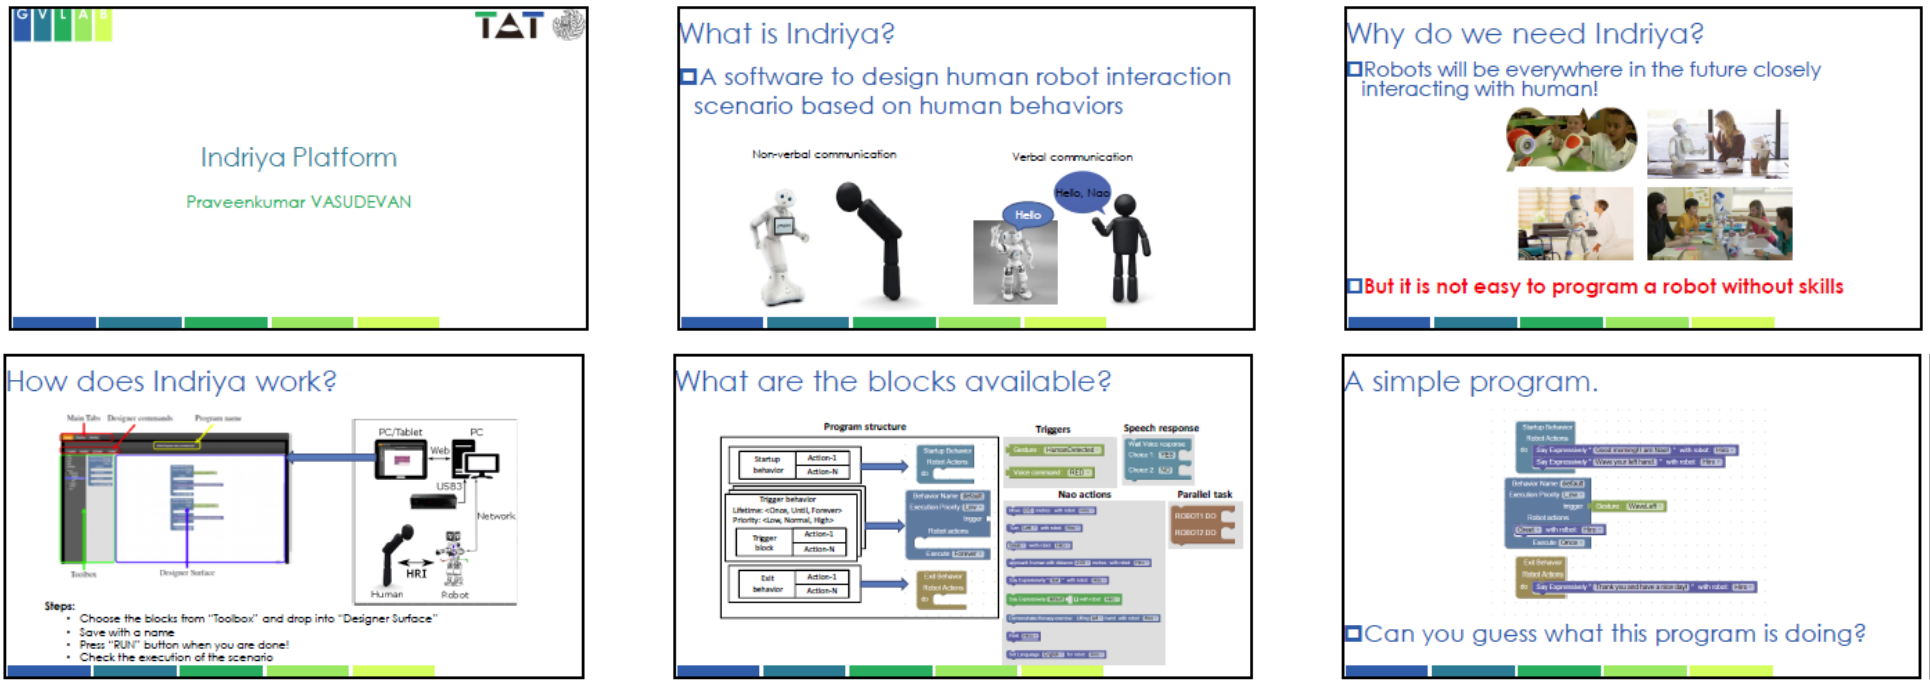
\includegraphics[width=\textwidth]{../thesis/assets/handout.png}
\caption[System description handout]{System description handout}
\label{fig:handout}
\end{figure}

The participants were given a short introduction about the system with the help of the handout. The participants were given a maximum of 90 minutes to think, design and execute the scenario designed using the Indriya platform. They were given a maximum of 2 chances to edit and execute the scenario on the real robot. Irrespective of whether they manage to complete what they desired at the end of two chances, they were asked to evaluate the system based on their experience of using it.

\section{Data collection method}
The self-assessment \cite{bethel2010review} technique has been used as the data collection method. A questionnaire has been framed in order to access various metrics of the user experience. The Google forms has been used to prepare the questionnaire. The questionnaire is at first made in English and after performing the pilot studies on a set of English speaking participants, it has been translated to Japanese with the help of a native Japanese speaker. The questionnaire has been integrated with the user interface. Soon after the participants design and execute the scenario, they could navigate to the \emph{Evaluate} screen (similar to the in-app rating system in modern applications) and evaluate the system. The Google forms integrated with user interface is shown in Fig.~\ref{fig:ui_evaluate}

\begin{figure}[H]
\centering
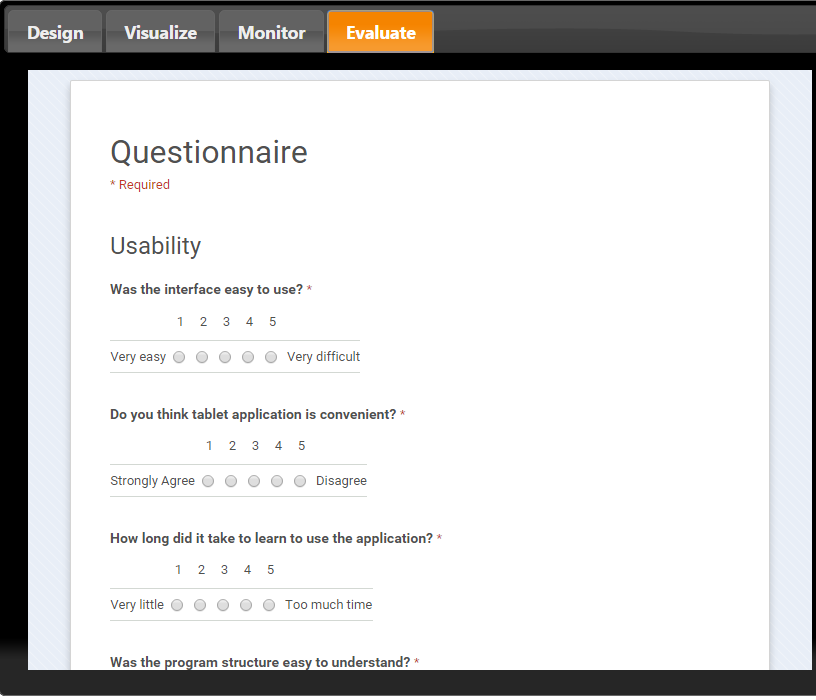
\includegraphics[width=0.7\textwidth]{../thesis/assets/questionnaire_integration.png}
\caption[Questionnaire integration in UI]{Questionnaire integration in UI}
\label{fig:ui_evaluate}
\end{figure}

The questionnaire is presented in Appendix~\ref{AppendixD}. Most of the questions in the questionnaire are based on Semantic differential scale in order to access the position of the user between two contrasting adjectives. The questionnaire has five sections namely
\begin{itemize}
\item Usability: To access the usability of the system
\item Execution: To access the performance of the system
\item System: To evaluate the overall capability of the system
\item Multi-robot programming: To access the usability of multi-robot programming
\item Background: To get an idea of the background of the users. However it is made sure that the sensitive information were not collected during the data collection.
\end{itemize}

\section{Data analysis}

\section{Summary and Discussion}
Thanks to the user study, apart from evaluating the system, several extreme cases and the functionalities an user expects out of the system were determined. The summary of the observations are
\begin{itemize}
\item Speech recognition: Many users suggested the usage of external microphone for the speech recognition. Most of the time during the interaction, the user is far away from the Kinect sensor so the voice recognition fails.
\item Exit behavior: The interpretation of exit behavior was different from user to user. It was observed that the participants had difficulty in observing when the life time of all configured blocks complete.
\item Triggers: Many users attempted to aggregate multiple triggers together to fire the execution of behavior block. Moreover some users also wanted to fire a behavior block with some variable. The users also wanted to execute the trigger behavior blocks until a gesture trigger arrives or wait until a gesture arrives to continue execution etc., While these capabilities were not supported at the time of conducting the experiments, it is very much possible to support all of these requirements from the user.
\end{itemize}